\label{chapter2}
\chapter{Fotometria, Colore e Camera}
\section{Fotometria}
L'occhio umano non \`e equamente sensibile a tutte le lunghezza d'onda della luce visibile, la quale \`e un sottoinsieme dello spettro elettromagnetico
corrispondente all'intervallo $[360,830] si{nm}$, come accennato nel primo capitolo \ref{chapter1}. Dunque, si introduce
\begin{definitionS}
	La \textit{Fotometria} \`e la scienza che studia la misurazione della luce in termini della \textit{intensit\`a percepita} dall'occhio umano.
\end{definitionS}
Tale definizione permette di capire che la fotometria si distingue dalla radiometria in quanto, data una sorgente luminosa $\Sigma$ con una certa
SPD, lo scopo \`e pesarne il contributo di ciascuna lunghezza d'onda secondo la percezione umana.\par
L'occhio umano possiede due tipi di fotorecettori: \textit{coni} e \textit{bastoncini}
\begin{itemize}[topsep=0pt, noitemsep]
	\item[] I \textit{coni} sono responsabili per la percezione in ambienti illuminati, detta \textit{visione fotopica}
	\item[] I \textit{bastoncini} sono responsabili per la percezione in ambienti bui, detta \textit{visione scotopica}
\end{itemize}
A seguito di esperimenti condotti nel 1931 dalla CIE, \`e stato associato un modello di risposta spettrale standard, e sono chiamate 
\textit{Efficacia Luminosa Spettrale Fotopica} $V_p(\lambda)$ e \textit{Efficacia Luminosa Spettrale Scotopica} $V_s(\lambda)$.\par
Tali funzioni, in ciascuna lunghezza d'onda, rappresentano un peso $\in[0,1]$, il quale pu\`o essere integrato con una grandezza radiometrica spettrale
per ottenere l'analoga grandezza fotometrica.\footnote{Si noti che tutte le formule viste finora per le grandezze radiometriche, come la relazione 
tra radianza e etendue \ref{chapter1:basicRadiance}, o le relazioni tra grandezze radiometriche}
\begin{align} \label{chapter2:photometricQuantities}
	\text{\Gls{Energia Luminosa} } Q_v &= K\int_\Lambda Q_{e,\lambda}(\lambda)V(\lambda)\mathrm{d}\lambda\\
	\text{\Gls{Flusso Luminoso} } \Phi_v &= K\int_\Lambda\Phi_{e,\lambda}(t, \lambda)V(\lambda)\mathrm{d}\lambda\\
	\text{\Gls{Illuminanza}|\Gls{Emittanza Luminosa} } E_v|M_v &= K\int_\Lambda E_{e,\lambda}|M_{e,\lambda}(\vec{p},\lambda)V(\lambda)\mathrm{d}\lambda\\
	\text{\Gls{Intensita Luminosa} } I_v &= K\int_\Lambda I_{e,\Omega,\lambda}(\hat{\omega},\lambda)V(\lambda)\mathrm{d}\lambda\\
	\text{\Gls{Luminanza}\footnotemark{} } Y &= K\int_\Lambda L_{e,\Omega,\lambda}(\vec{p},\hat{\omega},\lambda)V(\lambda)\mathrm{d}\lambda
\end{align}
dove $\Lambda = [380, 830] \si{nm}$, cio\`e intervallo nel quale le funzioni $V(\lambda) \neq 0$\\
\footnotetext{Nota come piuttosto che seguire la nomenclatura ISO per la Luminanza $L_v$ si \`e scelto di adottare $Y$. I motivi appariranno chiari 
nei cenni sulla colorimetria \ref{chapter2:section:colorimetry}}
Nota che non si \`e indicato quale funzione di efficacia luminosa si sta utilizzando, in quanto le formule sono universalmente valide. Le costanti,
invece, che rappresentano l'\textit{Efficacia Luminosa di una radiazione} cambiano valore:
\begin{itemize}[topsep=0pt, noitemsep]
	\item[] $K = 683.002\,\si{lm/W}$ Efficacia luminosa fotopica 
	\item[] $K \approx 1700\,\si{lm/W}$ Efficacia luminosa scotopica
\end{itemize}
Tali costanti rappresentano l'efficacia luminosa, cio\`e il fattore di conversione \mbox{$\si{W}\rightarrow\si{lm}$} per una radiazione monocromatica a
lunghezza d'onda $555 \si{nm}$.\par
\subsection{fotometria e sistemi di rendering}
La fotometria, nel contesto di Physically based Rendering, \`e utile per la modellazione di sorgenti luminose, per specificare parametri come 
intensit\`a luminosa, light falloff, e cos\`i via.\par
Includendo parametri fotometrici si pu\`o ottenere una descrizione pi\`u vicina all'uomo della percezione della luce mantenendone il rigore fisico.
\section{Colorimetria}\label{chapter2:section:colorimetry}
Il colore \`e un fenomeno la cui origine \`e sia fisica, determinato dalla distribuzione nelle lunghezze d'onda della radianza spettrale, sia 
psicobiologica, in quanto la sua percezione \`e artefatto dell'interpretazione di tali lunghezze d'onda nella corteccia cerebrale posteriore.\par
Ci\`o suggerisce che il colore \textit{non \`e una propriet\`a degli oggetti}, ma della luce da essi riflessa e dunque dipendente alle lunghezze d'onda
contenute nella radiazione incidente.\par
Nonostante specificare un colore sottoforma di spettro di frequenza del flusso radiante sia la modalit\`a pi\`u fedele e ottimale, essa
\begin{itemize}[topsep=0pt, noitemsep]
	\item Non \`e una interfaccia human-friendly e orientata alla percezione
	\item Non corrisponde alla rappresentazione utilizzata dai display odierni
\end{itemize}
Dunque, nel fornire un'interfaccia per un sistema di rendering, bisogna implementare la possibilit\`a di specificare colore in modo intuitivo, 
convertire tale specifica in uno spettro di frequenze per effettuare la computazione, e convertire nella rappresentazione nativa per mostrare a schermo
i risultati.\par
\begin{definitionS}
	Risulta dunque conveniente specificare delle \textit{funzioni di base} per poter costituire uno spazio vettoriale tramite il quale, specificandone
	i componenti, si specifica un determinato colore. Tale spazio vettoriale \`e chiamato \textit{Color Space}.
\end{definitionS}
\begin{figure}
	\centering
	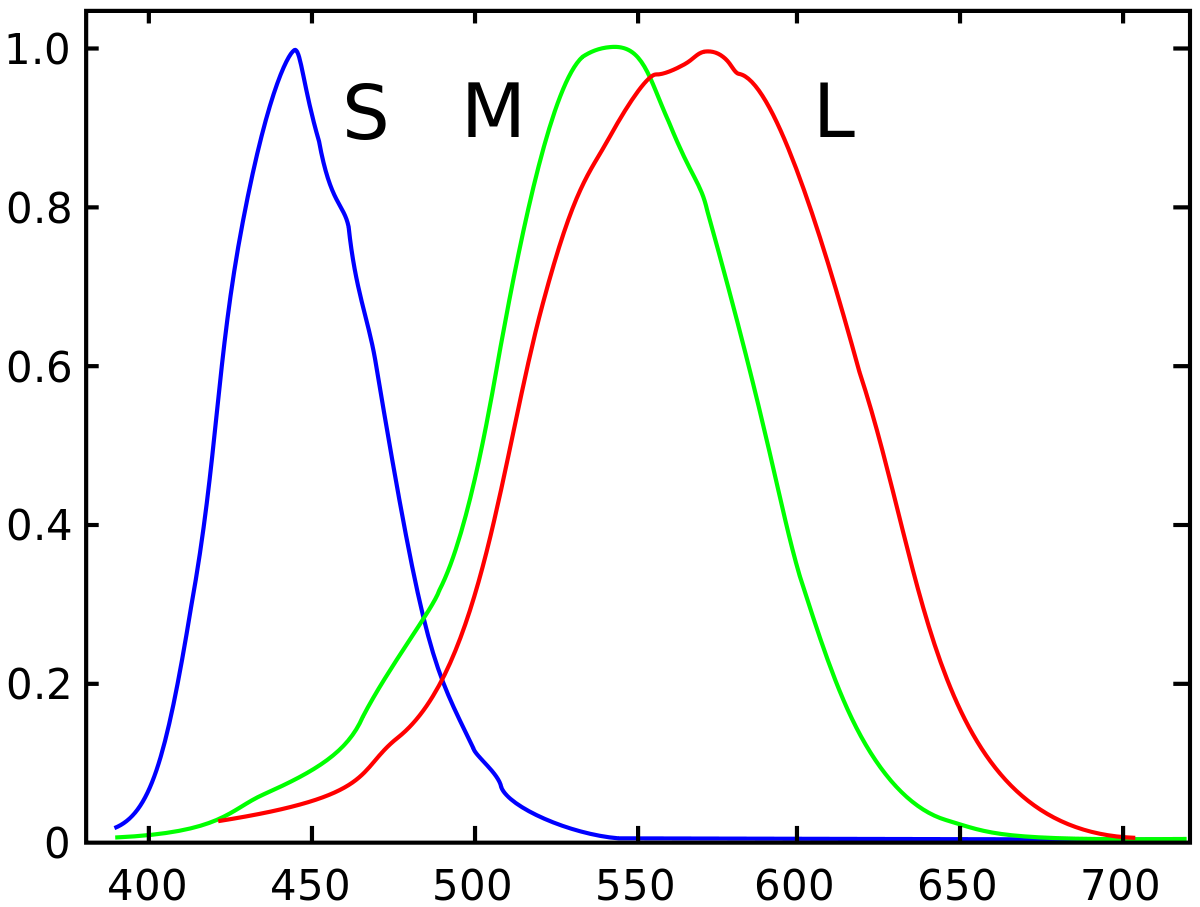
\includegraphics[width=0.4\textwidth]{../assets/chapter2_colorimetry_cones.png}
	\includesvg[width=0.55\textwidth, inkscapelatex=false]{../assets/chapter2_colorimetry_RGB_color_matching_functions.svg}
	\label{chapter2:figure:coneSpectralSensitivity}
	\label{chapter2:figure:RGBColorMatchingFunctions}
	\caption{\textit{A destra}, Sensibilit\`a spettrali per i tre tipi di coni dell'occhio umano. \textit{A sinistra}, color matching functions del 
			CIE 1931 RGB Color Space}
\end{figure}
Un \textit{color stimulus} pu\`o essere ricostruito dalla combinazione lineare da tre stimoli (distribuzioni spettrali) di base indipendenti 
[\cite{color}], in quanto dei fotorecettori umani che distinguono il colore, i coni, ce ne sono di \textit{tre tipi} (vedi figura 
\ref{chapter2:figure:coneSpectralSensitivity}). Tale mappa da SPD a \textit{tristimulus values} non \`e biunivoca, infatti, nei diversi color 
spaces che definiamo, esistono valori tristimolo che possono risultare dalla scomposizione di diverse SPDs. Tali colori 
sono detti \textit{metameri}.\par 
Dunque l'obiettivo \`e quello di ottenere distribuzioni spettrali $\langle R\rangle, \langle G\rangle, \langle B\rangle$ tali che ogni colore 
possa essere rappresentato come
\begin{equation}\label{chapter2:colorimetry:color}
	C = R\langle R\rangle + G\langle G\rangle + B\langle B\rangle
\end{equation}
tale compito non \`e scontato in quanto, da come si osserva in figura \ref{chapter2:figure:coneSpectralSensitivity}, quasi tutte le lunghezza d'onda 
stimolano con diversa intensit\`a almeno due tipi di coni. Dunque, nel 1931, fu derivato il CIE 1931 RGB Trichromatic system, cio\`e una terna di 
color matching functions $\bar{r}(\lambda)$, $\bar{g}(\lambda)$, $\bar{b}(\lambda)$, derivate compiendo dei test con un 
\textit{osservatore standard colorimetrico}, cio\`e limitando il field of view dei soggetti testati a $2^o$ dentro la fovea, per eliminare la 
variabilit\`a di percezione causata dal field of view dell'osservatore. Tali soggetti sono stati esposti a luci monocromatiche, i.e. i colori primari 
scelti, alle frequenze $700\,\si{nm}$ (rosso), $546.1\,\si{nm}$ (verde), $435.8\,\si{nm}$ (blu). L'intensit\`a di queste tre sorgenti primarie erano
tali che, se addizionate, restituiscono uno spettro costante la cui intensit\`a \`e pari alla Luminanza della sorgente complessiva 
\begin{align}
	R &= \int_\Lambda \bar{r}(\lambda)L_{e,\Omega,\lambda}(\lambda)\mathrm{d}\lambda\\
	G &= \int_\Lambda \bar{g}(\lambda)L_{e,\Omega,\lambda}(\lambda)\mathrm{d}\lambda\\
	B &= \int_\Lambda \bar{b}(\lambda)L_{e,\Omega,\lambda}(\lambda)\mathrm{d}\lambda\\
	L_v &= 1.0000 R + 4.5907 G + 0.0601 B\;[\si{cd/m^2}]
\end{align}
Le tre color matching functions (CMFs) cos\`i 
ottenute sono mostrate in figura \ref{chapter2:figure:RGBColorMatchingFunctions}.\par
Ai tempi della standardizzazione di un sistema tricromatico, in assenza di computers, risultava complicato fare calcoli con queste tre CMFs per via dei
lobi negativi. Dunque, sempre nel 1931, fu standardizzato il \textit{CIE 1931 XYZ Color System}, nel quale sono stati scelti tre 
\textit{primari immaginari}\footnote{non percepibili all'occhio umano} a partire dai primari del sistema CIE RGB 1931 in modo tale che
\begin{itemize}[topsep=0pt, noitemsep]
	\item uno spettro costante dia luogo a componenti $X = Y = Z$
	\item la componente $Y$ sia la luminanza della radiazione $Y = L_v$
	\item la CMF $\bar{y}$ sia uguale alla funzione di efficacia luminosa fotopica $\bar{y}(\lambda) = V_p(\lambda)$
	\item $Z$ \`e quasi uguale al blu di CIE RGB
	\item $X$ \`e un mix delle tre CMFs di CIE RGB
\end{itemize}
Dai requisiti la seguente trasformazione lineare \mbox{CIE RGB 1931 $\rightarrow$ CIE XYZ 1931} \`e stata ricavata
\begin{equation}\label{chapter2:colorimetry:RGB2XYZ}
	\begin{bmatrix}
		R \\ G \\ B
	\end{bmatrix}
	=
	\begin{bmatrix}
		2.768892 & 1.751748 & 1.130160 \\
		1.000000 & 4.590700 & 0.060100 \\
		0 & 0.056508 & 5.594292
	\end{bmatrix}
	\begin{bmatrix}
		X \\ Y \\ Z
	\end{bmatrix}
\end{equation}
La quale \`e anche valida per trasformare una CMF del sistema CIE RGB in una CMF del sistema CIE XYZ 1931.\par
Per passare da radianza spettrale ai tristimulus values, distinguiamo il caso in cui si sta analizzando una radiazione/superficie emissiva
\begin{align}
	X &= K\int_\Lambda L_{e,\Omega,\lambda}(\lambda)\bar{x}(\lambda)\mathrm{d}\lambda\\
	Y &= K\int_\Lambda L_{e,\Omega,\lambda}(\lambda)\bar{y}(\lambda)\mathrm{d}\lambda\\
	Z &= K\int_\Lambda L_{e,\Omega,\lambda}(\lambda)\bar{z}(\lambda)\mathrm{d}\lambda
\end{align}
Ed il caso in cui si sta analizzando un colore di una radiazione riflessa o trasmessa (fonti luminose secondarie)
\begin{align}
	X &= \frac{1}{\int_\Lambda L_{e,\Omega,\lambda}(\lambda)\bar{y}(\lambda)\mathrm{d}\lambda}
		\int_\Lambda S(\lambda)L_{e,\Omega,\lambda}(\lambda)\bar{x}(\lambda)\mathrm{d}\lambda\\
	Y &= \frac{1}{\int_\Lambda L_{e,\Omega,\lambda}(\lambda)\bar{y}(\lambda)\mathrm{d}\lambda}
		\int_\Lambda S(\lambda)L_{e,\Omega,\lambda}(\lambda)\bar{y}(\lambda)\mathrm{d}\lambda\\
	Z &= \frac{1}{\int_\Lambda L_{e,\Omega,\lambda}(\lambda)\bar{y}(\lambda)\mathrm{d}\lambda}
		\int_\Lambda S(\lambda)L_{e,\Omega,\lambda}(\lambda)\bar{z}(\lambda)\mathrm{d}\lambda\\
\end{align}
dove
\begin{equation}
	S(\lambda) = \left\{ \begin{aligned}
		R(\lambda)\;&\text{se riflessione}\\
		T(\lambda)\;&\text{se trasmissione}
	\end{aligned}\right.
\end{equation}
\subsection{xy chromaticity diagram}
\begin{figure}[tb]
	\includesvg[width=0.8\textwidth, inkscapelatex=false]{../assets/chapter2_colorimetry_chromaticity_diagram_1931.svg}
	\label{chapter2:colorimetry:cromaticityDiagram}
	\caption{xy Chromaticity Diagram del sistema tricromatico CIE XYZ 1931}
\end{figure}
Spesso si preferisce normalizzare i valori tristimolo per ottenere le \textit{coordinate di cromaticit\`a}
\begin{align}
	x = \frac{X}{X+Y+Z}\\
	y = \frac{Y}{X+Y+Z}\\
	z = \frac{Z}{X+Y+Z}
\end{align}
dove, in quanto $x+y+z=1$, soltanto le coordinate $xy$ sono necessarie per una completa descrizione del colore.\par
Il diagramma di cromaticit\`a \`e riportato in figura \ref{chapter2:colorimetry:cromaticityDiagram}. Il contorno curvo rappresenta l'insieme di punti
nel diagramma corrispondente alle radiazioni monocromatiche, mentre la curva evidenziata rappresenta il \textit{Luogo Planckiano}, insieme di punti
corrispondenti ad uno spettro di emissione di un corpo nero plankiano (formula \ref{chapter1:planckLaw}), con temperatura da $[1000,\infty]\,\si{K}$.
Parametro utile per descrivere ciascun punto del diagramma, in particolare quelli legati alle sorgenti luminose, \`e quello di
\begin{definitionS}
	La \textit{Temperatura di colore Correlata}(CCT) $T_{cp}$ \`e definita come temperatura del radiatore planckiano il cui colore percepito si
	avvicina di pi\`u allo stimolo dato nelle stesse condizioni di osservazione.\par
	Ci\`o si traduce nel trovare il punto nel luogo planckiano con distanza minima al punto di cromaticit\`a dato
\end{definitionS}
Altrettanto importanti nella specifica del diagramma di cromaticit\`a sono gli \textit{Illuminanti Standard}, sorgenti luminose teoriche con SPD e 
coordinate di cromaticit\`a note che approssimano determinate sorgenti luminose reali.
\begin{table}
	\begin{tabularx}{\linewidth}{cccY}
		\toprule
		Nome & CIE 1931 $2^o$ xy & CCT $\si{K}$ & Sorgente modellata\\
		\midrule
		A & $0.4476, 0.4075$ & $2856$ & Filamento di tungsteno incandescente\\
		D50 & $0.3457, 0.3585$ & $5003$ & Luce diurna all'orizzonte\\
		E & $\frac{1}{3}, \frac{1}{3}$ & $5454$ & SPD equienergia \\
		D55 & $0.3324, 0.3474$ & $5503$ & Luce diurna mattina/pomeriggio \\
		D65 & $0.3127, 0.3290$ & $6504$ & Luce diurna mezzogiorno\\
		\bottomrule
	\end{tabularx}
	\caption{Illuminanti standard CIE}
\end{table}
\subsection{sRGB color space}
Mentre per memorizzare image data un qualsiasi color space pu\`o essere utilizzato (infatti, si possono memorizzare anche dati relativi allo spettro 
direttamente [\cite{fichet}]), per mostrare colore a schermo si preferisce scegliere 3 primari ed un punto bianco, punto nel quale i 3 primari danno
contributo massimo. La scelta dei primari \`e guidata dalla percentuale di gamut che si desidera coprire con tutte le combinazioni lineari dei tre
primari scelti e limitazioni fisiche. Lo standard adottato per monitors e World Wide Web nel 1996 da IEC \`e \textit{sRGB}. Esso \`e un color space 
additivo basato sui tre primari rosso, verde, blu, e white point, le cui coordinate di cromaticit\`a sono riportate in tabella 
\ref{chapter2:colorimetry:sRGB}.\par
\begin{table}
	\begin{tabularx}{\linewidth}{ccccc}
		\toprule
		Cromaticit\`a & Rosso & Verde & Blu & White point(D65)\\
		\midrule
		$x$ & $0.64$ & $0.30$ & $0.15$ & $0.3127$\\
		$y$ & $0.33$ & $0.60$ & $0.06$ & $0.329$\\
		$Y$ & $0.2126$ & $0.7152$ & $0.0722$ & $1$\\
		\bottomrule
	\end{tabularx}
	\label{chapter2:colorimetry:sRGB}
	\caption{Coordinate degli stimoli primari e del white point del sRGB color space}
\end{table}
Altro componente per la specifica di un color space per un display \`e la funzione di trasferimento del display, in particolare 
\begin{definitionS}
	La \textit{electro-optical transfer function} (EOTF) \`e un funzione di trasferimento che converte un segnale immagine in input in intensit\`a 
	luminosa in output. Essa \textit{non \`e lineare}
\end{definitionS}
Tale funzione di trasferimento non \`e lineare per l'operazione di \textit{gamma correction} compiuta dai displays, la quale include sempre un 
elevamento a potenza $v_{in} = Av_{out}^\gamma$ (di solito $\gamma = 2.2$). Tale operazione \`e compiuta per ottimizzare l'uso dei bits 
nella codifica dell immagine, dando pi\`u importanza ai toni pi\`u scuri, in accordo con la percezione umana in grado di apprezzarli con 
pi\`u sensibilit\`a.\par
Dunque se l'output finale del sistema di rendering \`e un colore sRGB, dobbiamo essere capaci di convertire a/da un colore in sRGB color space da/a un
colore in XYZ color space. Sia $C_{srgb} = R_{srgb}|G_{srgb}|B_{srgb} \in [0,1]$ componenti del colore nello spazio sRGB gamma encoded. Simile
definizione per il colore nello spazio sRGB gamma corrected $C_{linear}$ ed il colore $[X, Y, Z]^T$ nello spazio XYZ.
\begin{equation}\label{chapter2:colorimetry:sRGB2XYZ}
	\text{Applica gamma correction: }C_{linear} = \left\{\begin{alignedat}{2}
		&\frac{C_{srgb}}{12.92}, &C_{srgb}\leq 0.04045\\
		&\left(\frac{C_{srgb}+0.055}{1.055}\right)^{2.4},\;&C_{srgb}> 0.04045
	\end{alignedat}\right.
\end{equation}
\begin{equation}
	\text{Applica trasformazione lineare\footnotemark{}: }\begin{bmatrix}
		X_{D65}\\ Y_{D65}\\ Z_{D65}
	\end{bmatrix}=
	\begin{bmatrix}
		0.4124 & 0.3576 & 0.1805 \\
		0.2126 & 0.7152 & 0.0722 \\
		0.0193 & 0.1192 & 0.9505 
	\end{bmatrix}
	\begin{bmatrix}
		R_{linear} \\ G_{linear} \\ B_{linear}
	\end{bmatrix}
\end{equation}
\footnotetext{i valori tristimolo X,Y,Z qui utilizzati/ottenuti sono scalati in modo tale che l'illuminante standard D65 abbia luminanza unitaria, 
cio\`e moltiplicate per $\approx 3.039513678$}
\subsection{Conversione da XYZ a SPD}
